\chapter{Aplicações, Considerações Finais e Conclusão}
Neste capítulo será discorrido acerca de algumas possibilidade de aplicações de NFP, encerrando com as principais conclusões que puderam ser extraídas deste trabalho bem como as considerações para trabalhos futuros que possam a vir ser realizados no âmbito do LabCEM do IFSC - Engenharia Eletrônica.

\section{Aplicações}
\subsection{Medidas de campo próximo}
A principal utilidade das NFPs esta na detecção de campo próximo afim de se efetuar análises de compatibilidade eletromagnética. Após a identificação de alguma frequência que esteja fora dos padrões e limites exigidos pelas normas, ou que interfira em algum tipo de susceptibilidade, muitas vezes se faz necessário rastrear no circuito a origem deste sinal espúrio, para isso existe o método de rastreamento utilizando uma NFP. 

Vimos nesse estudo que as NFPs desenvolvidas aqui em PCI, obtiveram excelentes resultados na detecção de frequências entre 5MHz até 25MHz (limites impostos pelos equipamentos disponíveis) para a verificação ponto a ponto, e, via analisador de espectro, viu-se que na faixa de 900MHz até 1.5GHz, temos uma resposta plana das NFPs desenvolvidas. Portanto, as NFPs desenvolvidas são viáveis a serem aplicadas na detecção de sinais espúrios via rastreamento por varredura.

\subsubsection{Produto Comercial}
Uma aplicação viável que foi vislumbrada durante a realização deste trabalho, foi quanto a prática comercial das NFPs desenvolvidas, dessa forma realizou-se uma comparação de resultados entre as características de resposta em frequência de uma NFP que está disponível comercialmente e algumas NFPs desenvolvidas neste trabalho. Na figura~\ref{fig:FD15CTeCOM} visualizamos as repostas para as versões FD15CT, FD30CT, FD60CT e uma NFP comercial, e notamos claramente que as NFPs desenvolvidas aqui possuem respostas tão boas quanto a NFP comercial investigada.

\begin{figure}[htb!]
	\centering 
	\caption{Resposta em Frequência - FD15CT, FD30CT, FD60CT e Comercial}
	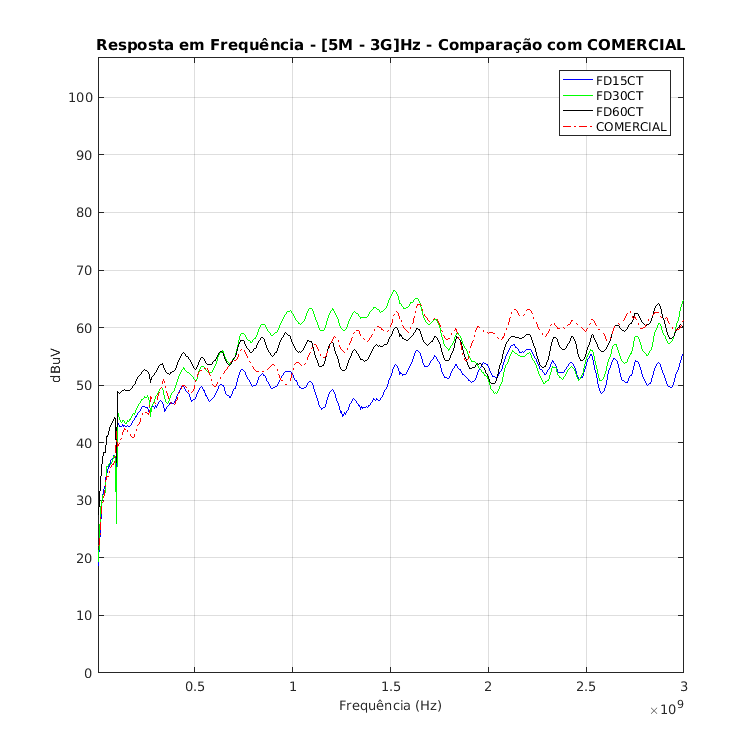
\includegraphics[scale=0.7]{./img/FD15CTeCOM}
	\fonte{Elaborado pelo Autor (2019)}
	%\legend{\hspace{-218pt}Fonte:~\citeonline[p.~8]{paul2006}}
	\label{fig:FD15CTeCOM}
\end{figure}

Diante deste fato, concluímos que as NFPs desenvolvidas em PCI são viáveis até para serem comercialmente trabalhadas, sendo que o preço de fabricação em PCI é mínimo. A título também de comparação buscou-se o valor praticado comercialmente na venda de pontas de prova de campo próximo e descobriu-se que frente ao custo de 1 conector SMA, 1 placa PCI de 10mm x 10mm e algumas horas trabalhadas (custo das NFPs aqui desenvolvidas) o preço comercial de NFPs em PCI daria uma margem de lucro muito alta. Na figura~\ref{fig:NFP_comercial_price} vemos que um kit com 4 NFP custa a monta de 295,00 (Duzentos e Noventa e cinco Dolares) o que equivale aproximadamente à 1150 (Mil Cento e Cinquenta Reais). Na figura~\ref{fig:NFP_comercial_meansure} visualizamos a NFP comercial investigada.

\begin{figure}[htb!]
	\centering
 	\caption{Preços e Medida - NFP Comercial}
	\subfloat[][Preço - NFP Comercial]{
		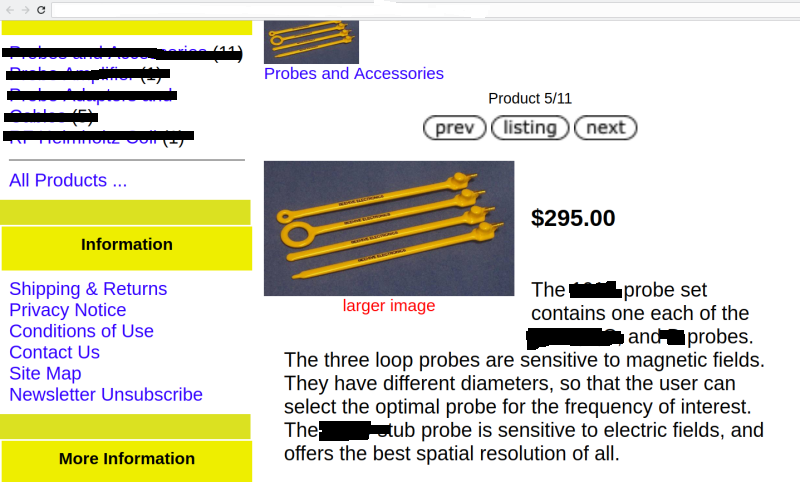
\includegraphics[scale=0.4]{./img/NFP_comercial_price}
		\label{fig:NFP_comercial_price}}
	\subfloat[][Medida - NFP Comercial]{
		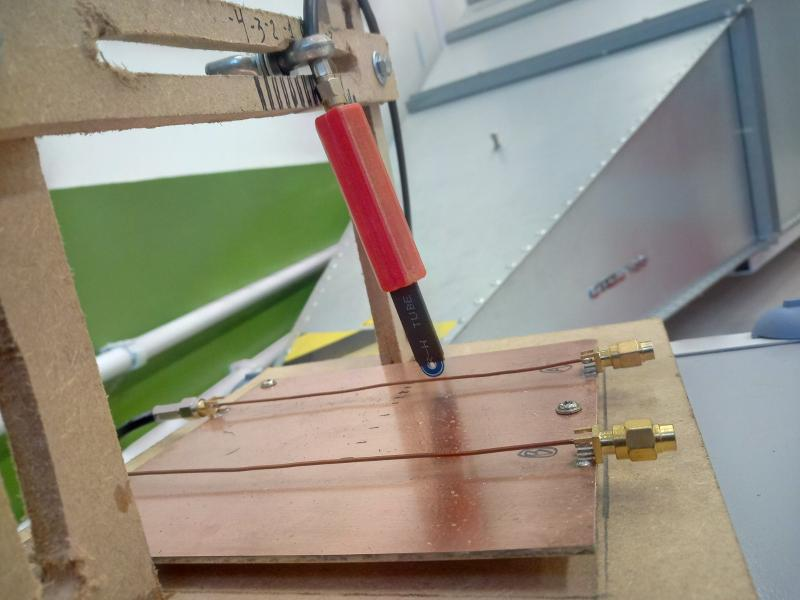
\includegraphics[scale=0.4]{./img/NFP_comercial_meansure}
		\label{fig:NFP_comercial_meansure}}
    \fonte{Elaborado pelo Autor (2019)}
\end{figure}

\subsection{Inserção de Campo Magnético}
Além de detectar, as NFPs são antenas e pelo principio da dualidade de antenas, as NFPs aqui desenvolvidas podem também serem aplicadas na inserção de campos magnéticos, no intuito de averiguar se a frequência do sinal inserido provoca algum tipo de anomalia ou defeito no DUT avaliado. Esta ação pode ser realizada juntamente com uma varredura, efetuando assim uma análise de compatibilidade eletromagnética do DUT e identificando a susceptibilidade ou não deste DUT à algum sinal espúrio que por ventura possa provocar defeitos.

%\subsubsection{Neuro Iteração}

\section{Considerações Finais}

\subsection{Aprimoramentos e Melhorias Necessárias}
% Sistema de medida precisa ser melhorado.. Necessário maior confiança no posicionamento.
Um dos principais pontos de melhorias é em relação ao sistema de posicionamento da NFP. Neste trabalho, conforme apresentado, utilizou-se um aparato em madeira cujo posicionamento foi feito manualmente, isso acarreta em erros de posicionamento e aumenta significativamente o tempo de medição. Sendo assim, seria de grande relevância para o LabCEM o desenvolvimento de um sistema automatizado de posicionamento das NFPs juntamente com um sistema eletrônico para aquisição dos dados.

Quanto aos leiautes desenvolvidos, poderia-se melhorar a disposição da carga resistiva e das vias de ligações entre uma face e outra (para as versões em face dupla), principalmente nas versões de NFP com raios pequenos (0.5mm, 1mm e 1.5mm). Isto seria possível utilizando métodos de fabricação de PCI comerciais com limites de \textit{clearance}, furação e trilhas mais sofisticados do que os disponíveis no IFSC, apesar do IFSC possuir ferramentas de fresa e métodos muito bons de fabricação de PCI, os limites são restritivos ao projetista, impondo certos limites de liberdade à escolha de um melhor posicionamento destes componentes.

\subsection{Dificuldades e Problemas Encontrados}
Uma das primeiras dificuldades encontradas foi na etapa de desenvolvimento e projeto das NFPs. As versões em face dupla necessitaram de uma via (interligação entre faces) além da carga resistiva para o casamento de impedância, e com isso, principalmente nos leiautes com raio menor que 1.5mm, teve-se dificuldades em alocar a via e projetar as espiras com volta completa. O caso de destaque aqui foram as versões FD05ST e FD05CT, cujo espira ficou no formato elíptico, isso acarretou em um comportamento levemente diferenciado em relação as demais.

% Equipamentos do LabCEM são Excelentes... mas na bibliografia utiliza-se muito um analisador de rede
Outra dificuldade, não tão impactantes, foi quanto ao uso de gerador de função e analisadores de espectro em falta de analisador de rede vetorial. Apesar de o LabCEM possuir excelentes equipamentos, nas referências adotadas é utilizando o analisador de rede vetorial nas caracterizações de intensidade por distância. O uso deste equipamento possibilitaria uma investigação em uma faixa muito maior de frequências e possibilitaria também algum tipo de investigação mais aprofundada quanto a ganhos e funções de transferências das NFPs desenvolvidas.

% Dificuldade para gerar frequências maiores que 25 MHz ... Geradores do IFSC vão no máximo a esta frequência
Por fim, apesar de termos apresentado a caracterização da resposta em frequência em uma faixa larga de 5MHz à 3GHz, nas investigações de intensidade por distância ficou-se limitado à máxima frequência disponível nos geradores de função dos laboratórios do IFSC, estabeleceu-se como faixa de investigação de 5MHz a 25MHz (limite máximo em frequência dos gerados disponíveis), isso não prejudicou o trabalho, porém uma análise mais ampla, principalmente na faixa de resposta plana das NFPs, não foi possível de se realizar.

\subsection{Perspectivas Futuras}
% Outras Topologias, Elipticas e Quadradas
O estudo e investigação realizada neste trabalho, não esgota as possibilidades de novas intervenções afim de cada vez mais esclarecer e entender o comportamento e resultados das pontas de prova de campo próximo. Um estudo que poderia ser realizado consequente a esse é quanto a utilização de outros formatos de topologias, como viu-se em dos casos aqui utilizou-se uma topologia elíptica (FD05ST e FD05CT) e esta apresentou em um resultado diferenciado em relação as outras, então, seria de grande valia um novo estudo e investigação quanto a diferentes topologias de espiras, como a elíptica e a quadrada.

% Modelagem matematica de um modelo de NFP.
Outro trabalho que poderia ser consequente a este, e um nível mais elevado e aprofundado, seria uma modelagem matemática com um equacionamento preciso da resposta e comportamentos de alguma topologia de ponta de prova de campo próximo, este trabalho estaria na vanguarda desta área e poderia trazer a tona uma equação precisa para projetos de NFPs.

% Software para simular medida em campo próximo.
Também caberia no futuro a elaboração de algorítimos que se propusessem a simular o comportamento e resultados de pontas de prova de campo próximo, afim de obter-se previamente resultados de simulação e assim confronta-los com resultados práticos coletados por sistemas de varredura automatizados.

% Estudar o custo de fabricação, desenvolvimento e a prática comercial destas NFPs... Montar um plano de negócios
Por fim, caberia também um estudo comercial de custos de fabricação e elaboração de algum plano de negócios quanto a exploração comercial destas NFPs, haja vista, como vimos, há hoje no mercado pontas de prova de campo próximo sendo comercializadas apenas no exterior (fora do Brasil) que entregam resultados similares aos obtidos com as pontas de prova em PCI aqui desenvolvidas.
	
\section{Conclusão}
%Estudar, Desenvolver e investigar experimentalmente topologias em placas de circuito impresso para sondas de campo próximo que sejam eficientes e de baixo custo para a obtenção de medidas de campo magnético próximo em análises de compatibilidade eletromagnética.

% Fator Antena
% Sensitividade
% Seletividade
% Resolução Espacial
% Largura de Banda

% Influência do Raio na Sensitividade
% Influência do plano de terra na sensibilidade e largura de banda
% 2 espiras na sensibilidade

%+ Espiras --> ++Sensitividade
%+ Plano de terra elimina ressonâncias, Diminui a Sensitividade (na banda passante) porém melhora a banda passante
%+ Para Raios grandes +Espiras não aumentam significativamente a sensibilidade
Através dos resultados obtidos na caracterização da resposta em frequência, podemos concluir que o número de espiras influencia diretamente na sensibilidade das NFPs, aumentando-a, algo previamente esperado conforme revisado no capítulo de fundamentação teórica e modelagem eletromagnética. Além disso, podemos verificar que a adição de um plano de terra insere uma capacitância de acoplamento ao terra que melhora significativamente a largura de banda para uma resposta plana em $dB \mu V$ das NFPs, porém, em contrapartida esse plano de terra diminui a sensibilidade. Por fim, nesta caracterização, notamos que o aumento do raio da espira também melhora a sensibilidade nos casos em que aumentamos de raios pequenos (0.5mm) para raios médios (1.5mm), porém para a situação de dobrar o raio de 3mm para 6mm não trouxe um aumento significativo na sensibilidade.

%Intensidade por distância
%+ Para Raios grandes temos boa sensibilidade, porém com o aumento da frequência diminui-se a resolução espacial, com plano de terra, diminui-se a resolução espacial (raios grandes)
%+ Raios grandes são bons para sensibilidade
Com os resultados obtidos na caracterização das intensidades pela distância, podemos notar, dentro da faixa analisada de 5MHz até 25MHz, que as NFPs de raios grandes (3mm e 6mm) possuem uma boa sensibilidade em toda a faixa analisada, porém aumentando-se a frequência perdemos a resolução espacial, pois começa-se a ter leituras altas de intensidade para posições cada vez mais afastadas, dessa forma, concluímos que NFPs com raios grandes são excelentes em sensibilidade porém perdem resolução espacial.

%    5MHz --> FD15ST (Melhor Resolução, não é mais sensitiva)
%    10MHz --> FD15ST (Melhor Resolução, não é mais sensitiva)
%    15MHz --> FD15ST (Melhor Resolução, não é mais sensitiva)
%    20MHz --> FD15ST (Melhor Resolução, não é mais sensitiva)
%    25MHz --> FD15ST (Melhor Resolução, não é mais sensitiva)
Outra indicação importante, extraída da caracterização das intensidades pela distância, foi que a versão FD15ST é a melhor versão em termos de resolução espacial na faixa analisada, obviamente que esta não foi a melhor versão em termos de sensibilidade, porém se o objetivo for a detecção de sinais espúrios, utilizando técnicas de varredura espacial, esta seria a NFP mais indicada, pois determinaria com o a melhor resolução espacial o ponto exato de emissão do sinal investigado.

%+ Espiras --> ++Sensitividade
%+ Plano de terra melhora a sensibilidade para baixas frequências nas versões de face simples
A caracterização da resolução espacial utilizando o DUT duplo serviu para corroborar os investigações previamente realizadas, com esta experimentação visualizou-se de fato que a versão FD15ST tem uma excelente resolução espacial e distingue satisfatoriamente duas frequências operando em simultâneo. Outros resultados interessantes deste experimento foi para a versão FD05ST que também apresentou uma boa resolução espacial, e neste caso, em especial, devemos relembrar que a topologia desta versão, em face de dificuldades de leiaute, ficou no formato de uma elipse, dessa forma, como já exposto para trabalhos futuros indica-se uma investigação mais acurada deste formato de espira.

%Falar das outras caracterisiticas (Fator de Antena Varia coma frequência, assim como os elementos modelados do circuito equivalente)

Neste trabalho teve-se por objetivo realizar um estudo, desenvolvimento e investigação experimental de topologias em placas de circuito impresso de sondas de campo próximo, e conclui-se que é possível confeccionar estas sondas de forma muito barata, utilizando apenas alguns milímetros quadrados de PCI um conector SMA, uma resistência SMD e algumas horas trabalhadas no desenho e confecção, obteve-se sondas com bons resultados quanto a detecção de campo magnético próximo, dessa forma, estas sondas estão aptas a serem utilizadas em métodos e técnicas voltadas à análise de compatibilidade eletromagnética.
